\documentclass[a4j,titlepage]{jarticle}
\usepackage{listings,jlisting}
\usepackage{color}
\usepackage{moreverb}
\usepackage{eclbkbox}
\usepackage{framed}
\usepackage[dvipdfmx]{graphicx}
\usepackage[top=30truemm,bottom=30truemm,left=15truemm,right=15truemm]{geometry}
\definecolor{OliveGreen}{rgb}{0.0,0.6,0.0}
\lstset{
  basicstyle={\ttfamily},
  identifierstyle={\small},
  commentstyle={\smallitshape \color[rgb]{0,0.5,0}},
  keywordstyle={\small\bfseries},
  ndkeywordstyle={\small},
  stringstyle={\small\ttfamily},
  frame={tb},
  breaklines=true,
  columns=[l]{fullflexible},
  numbers=left,
  xrightmargin=0zw,
  xleftmargin=0zw,
  numberstyle={\scriptsize},
  stepnumber=1,
  numbersep=1zw,
  lineskip=-0.5ex,
  linewidth=15cm
}
%ここまでソースコードの表示に関する設定




\title{テキスト処理}
\author{金子泰之\\情報理工学専攻 3年}
\date{2019年12月17日}
\begin{document}
\maketitle



\subsection*{5.1}
  課題5\_1text1からtext9までの語彙数\\
  text1: 17231\\
  text2: 6403\\
  text3: 2628\\
  text4: 9201\\
  text5: 5441\\
  text6: 1855\\
  text7: 11387\\
  text8: 882\\
  text9: 6349
\subsection*{5.2}
  課題5\_2 アルファベットの出現率と出現回数\\

  \begin{table}[htbp]
    \caption{text1からtext9までのアルファベットの出現回数}
    \scalebox{0.55}[1]{
    \begin{tabular}{lllllllllllllllllllllllllll}
    text&a & b & c & d & e & f & g & h  & i  & j  & k  &l   & m& n  &o   &p   &q   &r   &s & t  &u   &v   &w   &x   &y&z\\
    text1&77916& 16877& 22507& 38219& 117092& 20833& 20820& 62896& 65434& 1082& 8059& 42793& 23277& 65617&69326& 17255& 1556& 52134& 64231& 87996& 26697& 8598& 22222& 1030& 16872& 632\\
    text2&40446& 7938& 12443& 22323& 66609& 12227& 9552& 32264& 36524& 948& 2780& 20628& 14617& 38444& 42015& 7946& 604& 33246& 32772& 44995& 14717& 5849& 12655& 840& 11678& 69\\
    text3&15425& 2660& 2585& 9139& 19119& 3612& 2303& 13214& 8305& 488& 929& 5441& 3952& 11151& 10193& 1842& 17& 7628& 8613& 13515& 3556& 1353& 3085& 68& 2681& 108\\
    text4&46389& 9259& 20500& 23429& 83353& 17428& 10583& 31626& 47942& 949& 2003& 24269& 15159& 48231& 51636& 13941& 630& 40258& 39572& 62681& 19507& 7608& 11817& 1311& 10563& 626\\
    text5&11125& 1912& 3134& 3755& 13229& 1853& 2876& 7853& 10233& 1310& 2027& 6819& 4253& 9037& 12970& 3219& 60& 6568& 7255& 10709& 7405& 1041& 3427& 206& 4540& 225\\
    text6&4076& 859& 1281& 1658& 5092& 701& 1430& 3252& 2970& 64& 631& 2202& 1097& 2994& 3643& 621& 104& 3217& 2513& 3873& 1992& 428& 1032& 30& 1062& 33\\
    text7&33159& 6289& 14298& 15173& 46871& 8482& 8046& 16286& 29858& 848& 3052& 16349& 10727& 28884& 28980& 9195& 428& 27336& 28382& 36465& 11569& 3983& 5703& 1156& 6652& 314\\
    text8&1172& 195& 336& 638& 1798& 395& 512& 470& 1351& 33& 285& 898& 542& 1232& 1212& 335& 18& 948& 1275& 1015& 473& 185& 213& 19& 412& 4\\
    text9&21003& 3792& 6216& 10831& 30758& 5475& 5036& 15767& 17072& 182& 2267& 11019& 6500& 16239& 18374& 4250& 347& 13949& 16488& 22398& 7147& 2091& 5731& 311& 5769& 97\\
    \end{tabular}
    }
    \end{table}


  \fontsize{5.5pt}{0pt}\verbatimtabinput{./text/kadai5_2.txt}
  \newpage
  \begin{figure}[htbp]
    \begin{center}
      \begin{tabular}{c}
        \begin{minipage}{0.5\hsize}
          \begin{center}
            \fontsize{12pt}{5pt}\verbatimtabinput{./text/kadai5_2_.txt}
          \end{center}
        \end{minipage}
        \begin{minipage}{0.5\hsize}
          \begin{center}
            \fontsize{12pt}{5pt}\verbatimtabinput{./text/kadai5_2__.txt}
          \end{center}
        \end{minipage}
      \end{tabular}
      \caption{text1からtext9までのアルファベットの合計出現率}
    \end{center}
  \end{figure}


  \begin{center}
  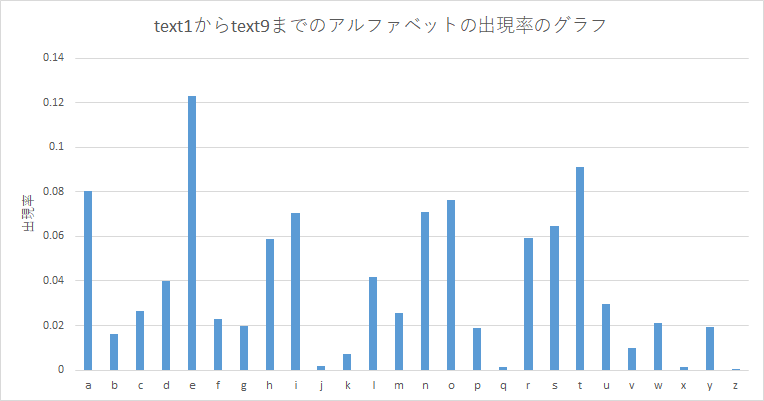
\includegraphics[width=14cm]{./kadai5_2_rate.png}
  \end{center}

\subsection*{5.3}
  課題5\_3 text1からtext9までの出現率上位5番目までの4文字以上の単語\\
  \fontsize{10pt}{5pt}\verbatimtabinput{./text/kadai5_3.txt}
  出現回数1位はthatであった。
\subsection*{5.4}
  課題5\_4 text1からtext9までのストップワードの比率\\
  \fontsize{10pt}{10pt}\verbatimtabinput{./text/kadai5_4.txt}
\subsection*{5.5}
  課題5\_5 wagahaiha\_nekodearu.txtに含まれる名詞の比率\\
  形態素解析を行いすべての品詞をすべて足したものを分母とし、分子は名詞の数とした。\\
  \fontsize{10pt}{10pt}\verbatimtabinput{./text/kadai5_5.txt}
\subsection*{5.6}
  課題5\_6 wagahaiha\_nekodearu.txtに含まれる出現頻度上位30位までの名詞\\
  \fontsize{10pt}{10pt}\verbatimtabinput{./text/kadai5_6.txt}
\subsection*{5.7}
  課題5\_7 wagahaiha\_nekodearu.txtにtop30\_jnounが含まれる頻度\\
  \fontsize{10pt}{10pt}\verbatimtabinput{./text/kadai5_7.txt}



\end{document}
